本章では関連研究について, 本研究の構成要素である 「Random Walk エンジン」「分散グラフ処理システム」「地理的分散環境におけるグラフ処理システム」の 3 つに分けて紹介する. その後, 本研究の位置づけを述べる. 

\section{Random Walk エンジン}\label{sec:Random Walk エンジン}

Random Walk (RW) はグラフ解析において頻繁に用いられるため, その RW 演算を効率的に実行するシステムの開発は有意義なものであり, 複数の既存技術が存在する. 

ThunderRW\cite{10.14778/3476249.3476257}, FlashMob\cite{10.1145/3477132.3483575} は共有メモリシステムにおける RW 演算の最適化を目的とした手法である. RW 演算ではランダムな隣接頂点への遷移を繰り返すため, 不規則なメモリアクセスが課題となる. そこで ThunderRW では異なる RW クエリの実行を切り替えることによりメモリアクセスの待ち時間を隠蔽した. また FlashMob では, Random Walker (RWer) は高次数頂点に高頻度で訪れることに注目し, 高次数頂点の隣接辺の事前サンプリングを行うことで, RWer の遷移を DRAM への Sequential Read に置き換え, メモリアクセスのオーバヘッドを削減した. 

DrunkardMob\cite{10.1145/2507157.2507173}, GraphWalker\cite{254449}, NosWalker\cite{10.1145/3582016.3582025} はシングルマシンで動作する Out-of-Core RW エンジンである. Out-of-Core RW エンジンでは, 全てのグラフデータをメモリに載せて演算を行うのではなく, 必要なグラフデータを逐一メモリにロードしながら RW 演算を実行する. DRAM に対して低価格である SSD を利用してグラフデータを保持するため, 大規模グラフ上における RW 演算をより低コストで実行することが可能になる. NosWalker では, エッジサンプリングはエッジデータのみ, walker のアップデート処理は頂点データのみが必要となる RW の特性に注目し, それぞれの処理を分離する walker 指向の非連結アーキテクチャを採用している. 
% 最先端手法である NosWalker は, 汎用的な Out-of-Core グラフ処理フレームワークをベースとしている DrunkardMob, GraphWalker に対し, RW の特性を活かしたアーキテクチャを採用している.

KnightKing\cite{10.1145/3341301.3359634} はグラフデータを分散クラスタ上で保持する分散グラフ RW エンジンである. KnightKing には汎用性の高い API が設定されており, PPR, DeepWalk, MetaPath, Node2vec といった複数種類の RW を実行することができる. さらに KnightKing の貢献として, rejection ベースのエッジサンプリング手法による, 高次 RW アルゴリズムのコスト削減がある. RW 演算のボトルネックはエッジのサンプリング処理にあると言われており, walker の現在の状態, 前回訪れた頂点, 現在滞在している頂点のエッジの性質に依存するような動的サンプリングを必要とする高次 RW は顕著にその傾向を示している. KnightKing の rejection ベースのエッジサンプリングは O(d) (d: 頂点における次数)かかっていたエッジの動的サンプリングを O(1) (前計算 O(n), n: 頂点数) に削減した.

\section{分散グラフ処理システム}

近年のグラフデータの増加に伴い, 分散クラスタ上で動作する分散グラフ処理システムの重要性が高まっている. 分散グラフ処理における主流なプログラミングモデルとして, Bulk Synchronous Parallel (BSP) モデルがある. BSP モデルは, スーパーステップと呼ばれる単位で処理を繰り返し行うモデルであり, このスーパーステップは主に
\begin{itemize}
    \item サーバごとでの計算
    \item サーバ間同期
\end{itemize}
で構成される. 同期型である BSP モデルを非同期型にすることで処理を高速化する手法も存在する\cite{BAP}\cite{AAP}\cite{Gluon-Async}が, 実装の複雑化や, データセンター内等の広帯域環境では同期のオーバヘッドがさほど大きくならないことから, BSP モデルが採用されることが多い. 

BSP モデルの分散グラフシステムのうち, 頂点の状態に注目した手法\cite{Pregel}\cite{10.1145/2741948.2741970}\cite{10.5555/2387880.2387883}\cite{10.5555/3026877.3026901}\cite{Gluon}は vertex-centric なモデルと呼ばれる. vertex-centric モデルにおける各スーパーステップでは, 各頂点が, 直前のスーパーステップで送られたメッセージに基づいて自身の状態を更新し, 結果を他の頂点に送信する. ユーザは頂点における更新に関する処理を記述するのみであり, PageRank, Single Source Shortest Path, connected components 等の多くのグラフアルゴリズムはこの vertex-centric の形で書き下すことが可能である. 

対して\ref{sec:Random Walk エンジン}で紹介した KnightKing は, 処理単位が RWer であることから walker-centric モデルと呼ばれている. 図\ref{walker centric モデルの概要} は walker-centric モデルの概要を示しており, 各スーパーステップでは, 
\begin{itemize}
    \item 各 RWer がユーザー定義の RW を実行 (1 ステップ進める) し, 状態を更新
    \item 状態を更新した RWer の内, 他のサーバが管理する頂点へ遷移した RWer を送信し, 全サーバで同期
\end{itemize}
を行う. vertex-centric モデルを採用しないのは, RW における RWer の概念は, 既存の vertex-centric モデルのシステムではメッセージとして扱われるため, RWer の状態更新の追跡や最適化のための機能が失われる可能性が高いためである. 

\begin{figure}[t]
    \centering
    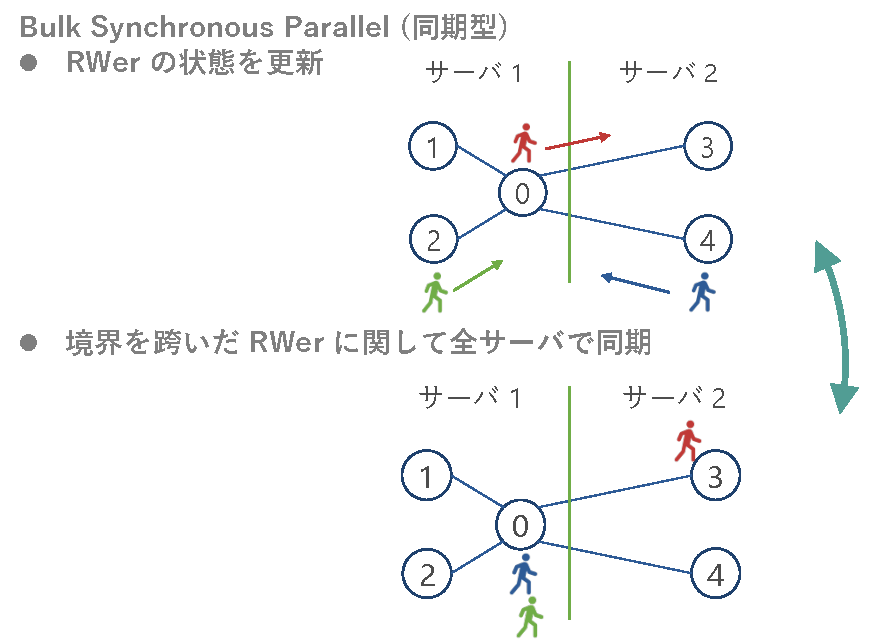
\includegraphics[scale=0.7]{figure/walkercentric.pdf}
    \caption{walker centric モデルの概要}
    \label{walker centric モデルの概要}
\end{figure}

\section{地理的分散環境におけるグラフ処理システム}

\section{本研究の位置づけ}